% ****** Start of file aapmsamp.tex ******
%
%   This file is part of the AAPM files in the AAPM distribution for REVTeX 4-2.
%   Version 4.2a of REVTeX, January 2015
%
%   Copyright (c) 2015 American Association of Physicists in Medicine (AAPM).
%
%   See the AAPM README file for restrictions and more information.
%
% TeX'ing this file requires that you have AMS-LaTeX 2.0 installed
% as well as the rest of the prerequisites for REVTeX 4.2
%
% It also requires running BibTeX. The commands are as follows:
%
%  1)  latex  aapmsamp
%  2)  bibtex aapmsamp
%  3)  latex  aapmsamp
%  4)  latex  aapmsamp
%
% Use this file as a source of example code for your aapm document.
% Use the file aapmtemplate.tex as a template for your document.
\documentclass[%
 aapm,
 mph,%
 amsmath,amssymb,
%preprint,%
 reprint,%
%author-year,%
%author-numerical,%
]{revtex4-2}
\usepackage{amssymb}
\usepackage{graphicx}
\usepackage{hyperref}
\usepackage{listings}
\usepackage{mathtools}
\usepackage{maple}
\usepackage[utf8]{inputenc}
\usepackage[svgnames]{xcolor}
\usepackage{amsmath}
\usepackage{breqn}
\usepackage{textcomp}
\usepackage{subcaption}
\usepackage[settings]{markdown}


% \begin{document}
\lstset{basicstyle=\ttfamily,breaklines=true,columns=flexible}
\pagestyle{empty}
\DefineParaStyle{Maple Bullet Item}
\DefineParaStyle{Maple Heading 1}
\DefineParaStyle{Maple Warning}
\DefineParaStyle{Maple Heading 4}
\DefineParaStyle{Maple Heading 2}
\DefineParaStyle{Maple Heading 3}
\DefineParaStyle{Maple Dash Item}
\DefineParaStyle{Maple Error}
\DefineParaStyle{Maple Title}
\DefineParaStyle{Maple Ordered List 1}
\DefineParaStyle{Maple Text Output}
\DefineParaStyle{Maple Ordered List 2}
\DefineParaStyle{Maple Ordered List 3}
\DefineParaStyle{Maple Normal}
\DefineParaStyle{Maple Ordered List 4}
\DefineParaStyle{Maple Ordered List 5}
\DefineCharStyle{Maple 2D Output}
\DefineCharStyle{Maple 2D Input}
\DefineCharStyle{Maple Maple Input}
\DefineCharStyle{Maple 2D Math}
\DefineCharStyle{Maple Hyperlink}


\usepackage{gensymb}
\usepackage{graphicx}% Include figure files
\usepackage{dcolumn}% Align table columns on decimal point
\usepackage{physics}
% \usepackage{mathtools}
% \usepackage{amsmath}
\usepackage{bm}% bold math
\usepackage[mathlines]{lineno}% Enable numbering of text and display math
\usepackage{multirow}
\usepackage[normalem]{ulem}
\useunder{\uline}{\ul}{}
\modulolinenumbers[5]% Line numbers with a gap of 5 lines

\begin{document}
\noindent
\header{ENGR 120}
%\preprint{AAPM/123-QED}

\title[]{\underline{Fluid Mechanics: Lab 5} \\
Venturi and Orfice flow measurements and characterization}.% Force line breaks with \\

\author{Christian Emil Lorentsen}%
\author{Serafin Stauch}
\author{Bryan Saldivar}
\author{Xuan Zhao}

\affiliation{University of California, Merced}
\date{\today}% It is always \today, today,
             %  but any date may be explicitly specified
\begin{abstract}
In this report we take a look at the Ventury and Orifice meter to determine the volume flow rate through a pipe. This is done from two simple pressure measurements, at two different points in the pipe. We also apply the steady flow energy equation to our systems, to study the friction head loss in the meters, by measuring the pressure at three different points. Finally we also study the discharge coefficient in the Orifice meter.

\end{abstract}

\maketitle
\linenumbers\relax % Commence numbering lines
\begin{quotation}
%Explain why the physics you are studying is interesting and relevant.
Venturi and Orifice meters provides and excellent way of measuring volume flow rate. From two simple pressure reading it is possible to measure the volume flow rate in a pipe using a Venturi meter, making it useful in a large variety of application. An Orifice meter also makes us able to measure the flow rate through a pipe, this time only using a small hole.

\end{quotation}
\section{\label{sec:level1}Background}
First, we look at the Venturi meter. It consists of a circular pipe, with a given volume flow rate. At a section of the pipe, where it conically shrinks shortly, we measure the pressure at three different points, see fig \ref{fig:Venturi}. The Orifice meter is almost identical to the Venturi meter, although there is no conical shrinkring, but a \textit{wall} with a small hole in the middle of diameter $d$, see fig \ref{fig:Orifice}.

\subsection{\label{sec:level2}Theory}
From Bernoullis eq. we get the following for the Venturi meter:

\begin{eqnarray}
P_a +\frac{1}{2} V_a^2 + \rho g z_a = p_b + \frac{1}{2} \rho V_b ^2 + \rho g z_1 \\
\Rightarrow A_b^2 P_V = \frac{1}{2}A_b^2 \rho \big(V_b^2 - \tfrac{d_a^4}{d_b^4}V_b^2 \big) 
\end{eqnarray}
Where we get $V_a = (d_b^2/d_a^2)V_b$ from conservation of mass. This leads to the following equations:
\begin{eqnarray}
    Q = \frac{\pi}{4}d_b^2 \sqrt{\frac{2P_v}{\rho(1-d_a^4/d_b^4)}} \\
    P_v = \frac{8Q^2\rho(1-d_a^4/d_b^4)}{\pi^2d_b^2}
    \label{eq:Qventuri}
\end{eqnarray}

Eq. 373\cite{White_Xue_2021}
\begin{equation}
    \bigg(\frac{p}{\gamma} + \frac{V^2}{2g} + z\bigg)_{in} = \bigg(\frac{p}{\gamma} + \frac{V^2}{2g} + z\bigg)_{out} + h_{friction}
\end{equation}
Since we have no pump or turbine. $z_{in}=z_{out}$ and applying between point A and B we get
\begin{eqnarray}
    h_{f1} = \frac{P_v}{\rho g} + \frac{1}{2g}(V_a^2-V_b^2) = \frac{P_v}{\rho g} + \frac{Q^2}{2gA_b^2}\bigg(\frac{d_b^4}{d_a^4}-1\bigg) \\
    = \frac{P_v}{\rho g} + \frac{2Q^2}{g\pi^2d_b^4}\bigg(\frac{d_b^4}{d_a^4}-1\bigg)
    \label{eq:hf1}
\end{eqnarray}
It is easy to apply it between point A an C, since they have the same crossectional area, and we loose the second term:
\begin{eqnarray}
    h_{f2} = \frac{P_d}{\rho g}
    \label{eq:hf2}
\end{eqnarray}
For the Orifice plate the relationship between the flow rate and pressure drop can be derived as \cite{White_2021}
\begin{eqnarray}
    Q = C_d A_t \bigg[\frac{2\Delta p}{\rho(1-\beta^4)}\bigg]
    \label{eq:Cd}
\end{eqnarray}
Where $C_d$ is the discharge coefficient, $A_t$ is the throat area and $\beta = d/D$, see fig \ref{fig:Orifice}
\subsection{\label{sec_level3}Method \& Setup}



For both the Venturi and Orifice meter we choose 6 values of $Q$ and measure $P_d$, $P_v$ and $\Delta p$ as seen in fig \ref{fig:setup}

\begin{figure}[h!]
  \begin{subfigure}{0.51\columnwidth}
    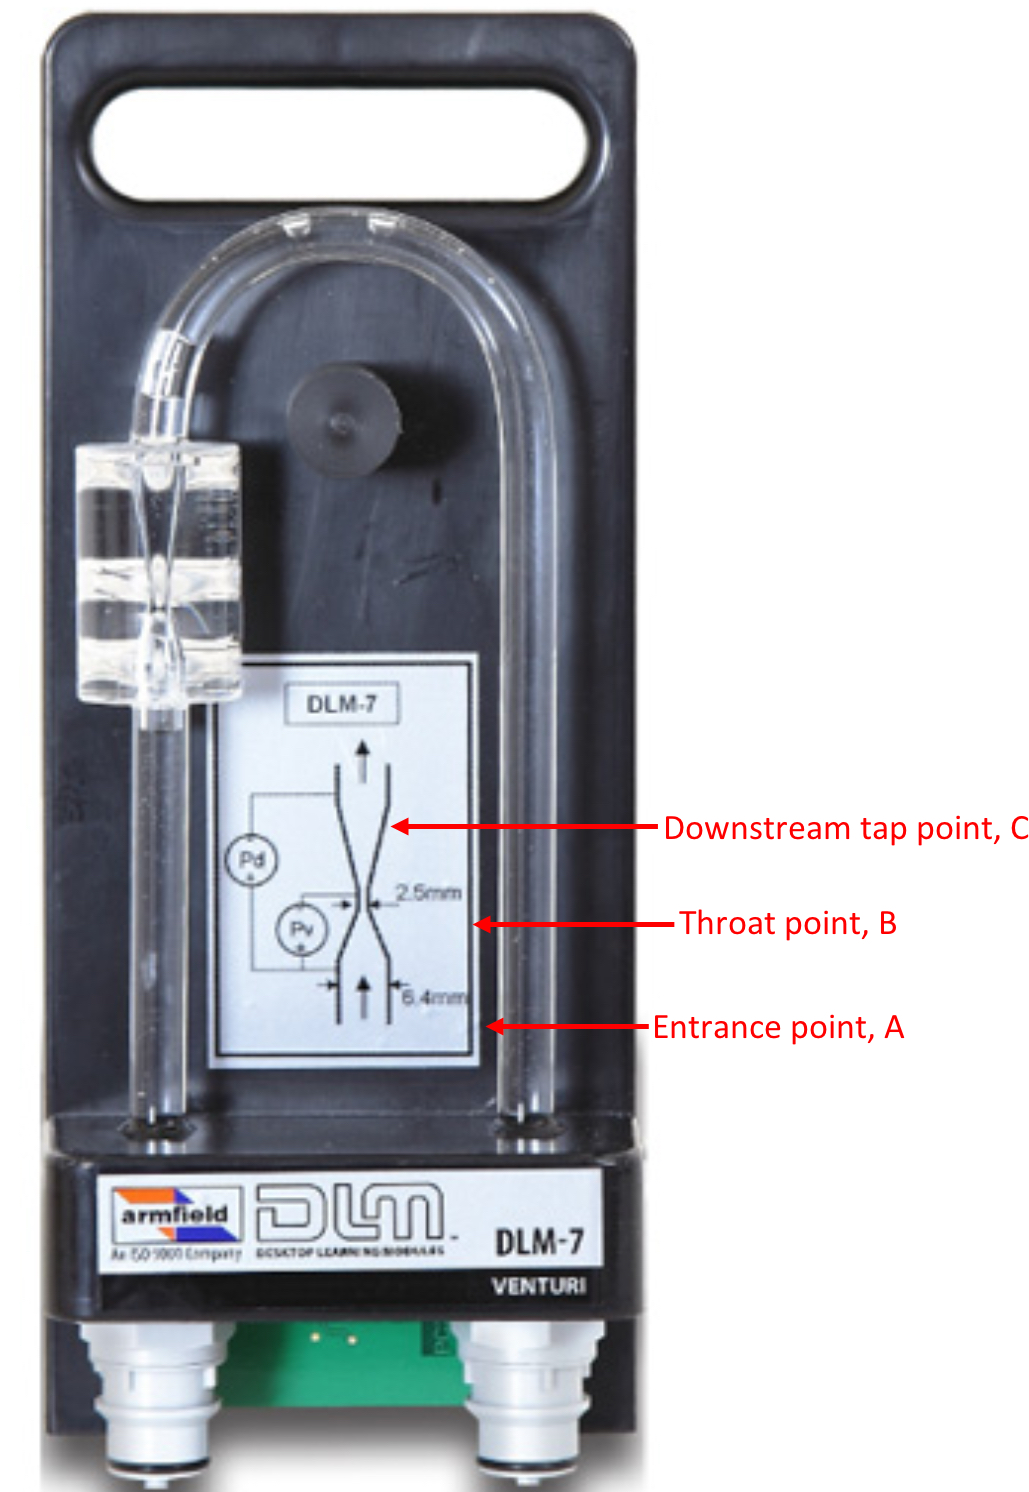
\includegraphics[width=\linewidth]{Diagrams/Venturi.jpeg}
    \caption{Venturi meter} 
    \label{fig:Venturi}
  \end{subfigure}%
  \hspace*{\fill}   % maximize separation between the subfigures
  \begin{subfigure}{0.435\columnwidth}
    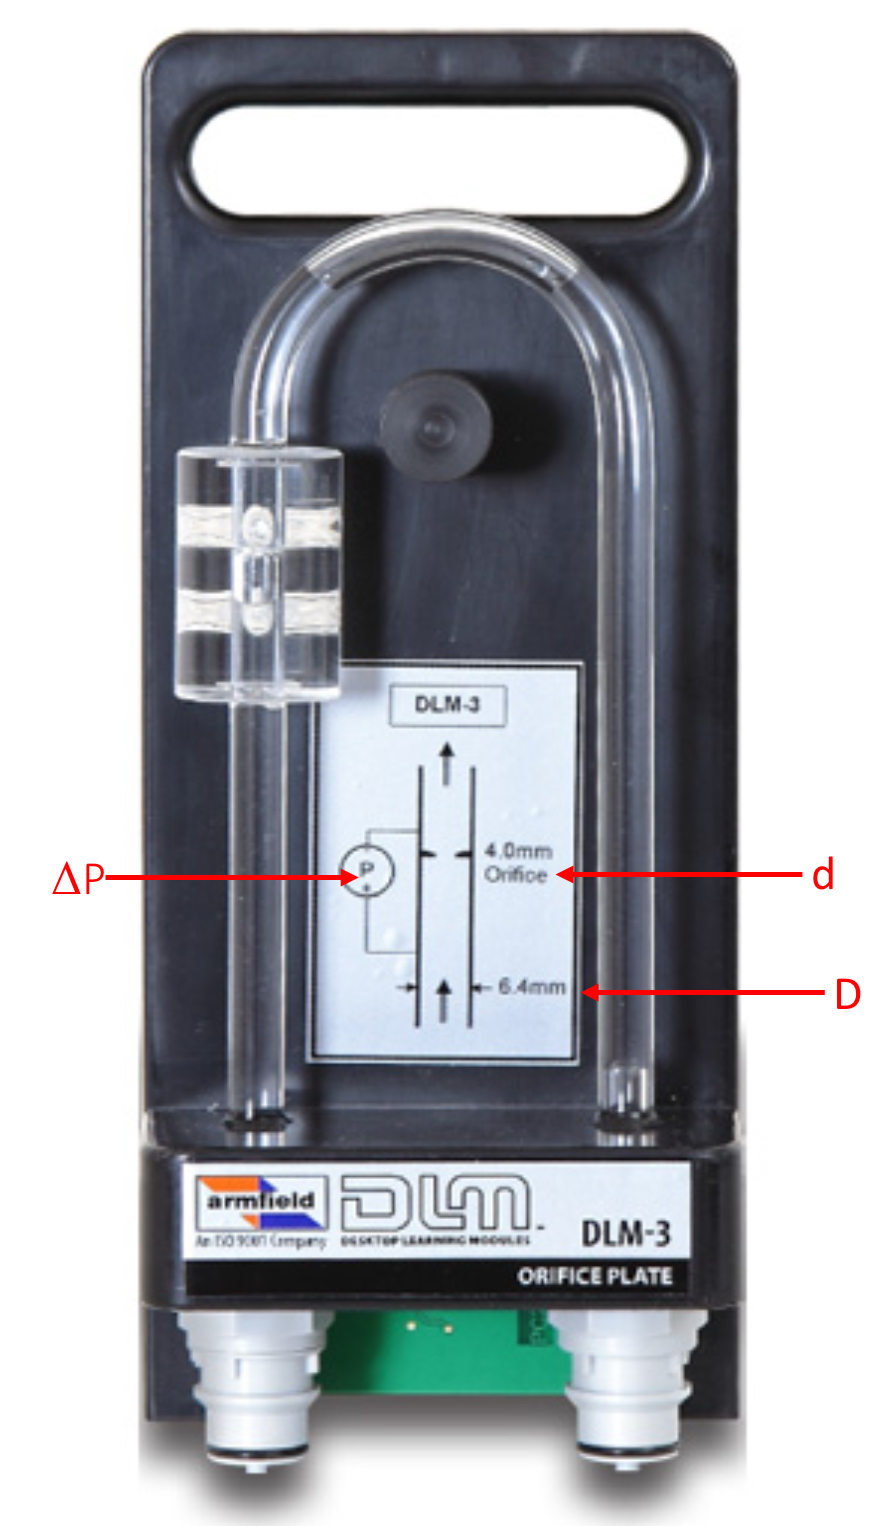
\includegraphics[width=\linewidth]{Diagrams/Orifice.jpeg}
    \caption{Orifice meter} 
    \label{fig:Orifice}
  \end{subfigure}%

\label{fig:setup}
\caption{Overview of the two different systems in use} \label{fig:Meters}
\end{figure}

\newpage
\section{DATA AND RESULTS}
% \textbf{Fra Jasons slides:} \\
% \textit{
% Include the data you took as figures or tables. \\
% Any figures and tables should have appropriate captions and must be referenced somewhere in the main text. \\
% Be sure that the plots are properly formatted with axes labels, units, and any relevant error bars on data. 
% }

Listed in Table \ref{table:Data} are the values measured from the setups described in \ref{sec_level3}. Also there are calculated values, where the Ideal $P_v$ is calculated using eq. \ref{eq:Qventuri} and $C_d$ from eq. \ref{eq:Cd}

% Please add the following required packages to your document preamble:
% \usepackage{graphicx}
\begin{table}[h!]
\resizebox{\columnwidth}{!}{%
\begin{tabular}{l|lll|ll|}
\cline{2-6}
                                           & \multicolumn{3}{l|}{Venturi Meter}                                                                              & \multicolumn{2}{l|}{Orifice meter}                                        \\ \hline
\multicolumn{1}{|l|}{\textbf{Q $[m^3/s]$}} & \multicolumn{1}{l|}{Measured $P_v [Pa]$} & \multicolumn{1}{l|}{\textbf{Measured $P_d [Pa]$}} & Ideal $P_v [Pa]$ & \multicolumn{1}{l|}{\textbf{$\delta p [Pa]$}} & \textbf{Calculated $C_d [m^{-1}]$} \\ \hline
\multicolumn{1}{|l|}{$16.67*10^{-6}$}         & \multicolumn{1}{l|}{$-5350$}             & \multicolumn{1}{l|}{$-3450$}                      & $-241.8$         & \multicolumn{1}{l|}{$1850.00$}                & $0.63$                    \\ \hline
\multicolumn{1}{|l|}{$25.00*10^{-6}$}         & \multicolumn{1}{l|}{$-9950$}             & \multicolumn{1}{l|}{$-5950$}                      & $-544.0$         & \multicolumn{1}{l|}{$4050.00$}                & $0.64$                    \\ \hline
\multicolumn{1}{|l|}{$33.33*10^{-6}$}         & \multicolumn{1}{l|}{$-17400$}            & \multicolumn{1}{l|}{$-8850$}                      & $-967.2$         & \multicolumn{1}{l|}{$7200.00$}                & $0.64$                    \\ \hline
\multicolumn{1}{|l|}{$41.67*10^{-6}$}         & \multicolumn{1}{l|}{$-27200$}            & \multicolumn{1}{l|}{$-12250$}                     & $-1511.2$        & \multicolumn{1}{l|}{$11450.00$}               & $0.64$                    \\ \hline
\multicolumn{1}{|l|}{$50.00*10^{-6}$}         & \multicolumn{1}{l|}{$-38200$}            & \multicolumn{1}{l|}{$-16300$}                     & $-2176.2$        & \multicolumn{1}{l|}{$16550.00$}               & $0.64$                    \\ \hline
\multicolumn{1}{|l|}{$58.33*10^{-6}$}         & \multicolumn{1}{l|}{$-49650$}            & \multicolumn{1}{l|}{$-20650$}                     & $-2962.0$        & \multicolumn{1}{l|}{$23350.00$}               & $0.62$                    \\ \hline
\end{tabular}%
}
\caption{Data for Venturi meter with an average value for $C_d\approx0.636 $.}

\label{table:Data}
\end{table}



% Please add the following required packages to your document preamble:
% \usepackage{graphicx}

\subsection{Analysis}
If we were to (hypothetically) measure a pressure drop of $6.35 mbar$ across the orfice plate with $C_d \approx 0.363 m^{-1}$ you would get a volume flow rate of $Q\approx 9.80\cdot 10^{-6} m^3/s$
\begin{figure}[h!]
    \centering
    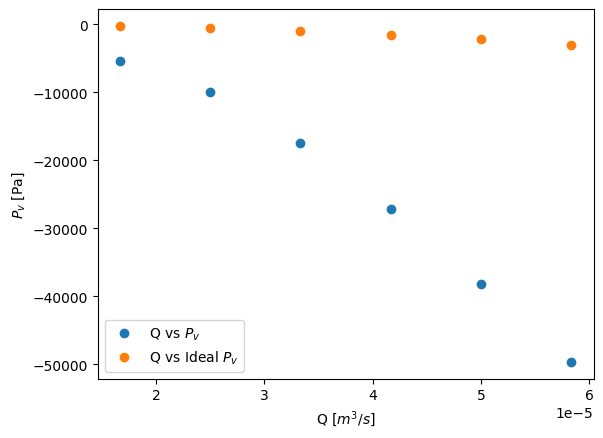
\includegraphics[width=60mm]{Diagrams/PvVsQ.png}
    \caption{Plot of measured $p_v$ vs $Q$ and and ideal $p_v$ vs $Q$}
    \label{fig:pvVsQ}
\end{figure}

\begin{table}[h!]
\resizebox{\columnwidth}{!}{%
\begin{tabular}{lr}
\toprule
h & Q \\
\midrule
$0.140 \pm 0.010$ & 0.00 \\
$0.160 \pm 0.010$ & 0.00 \\
$0.180 \pm 0.010$ & 0.00 \\
$0.190 \pm 0.010$ & 0.00 \\
$0.150 \pm 0.010$ & 0.00 \\
$0.190 \pm 0.010$ & 0.00 \\
\bottomrule
\end{tabular}

}
\caption{Table of calculated  \ref{eq:hf1} and \ref{eq:hf2}}
\label{table:hf1hf2}


\end{table}


\begin{figure}[h!]
    \centering
    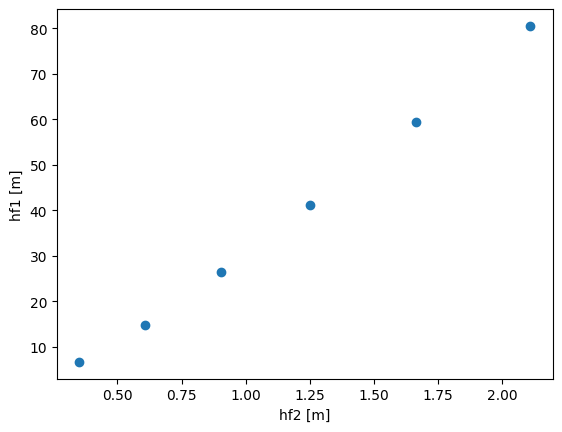
\includegraphics[width=60mm]{Diagrams/hf1Vshf2.png}
    \caption{Plot of $h_{f1}$ vs $h_{f2}$}
    \label{fig:hf1Vshf2}
\end{figure}


\begin{figure}[h!]
    \centering
    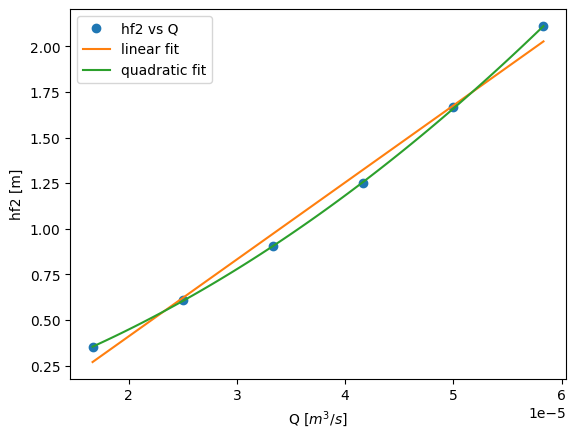
\includegraphics[width=60mm]{Diagrams/hf2VsQ.png}
    \caption{Plot of $h_{f2}$ vs $Q$ Including both linear $(a\cdot x+b)$ and quadratic fit$(a\cdot x^2 + b\cdot x^2 +c )$}
    \label{fig:hf2VsQ}
\end{figure}


% \textbf{Fra Jasons slides:} \\
% \textit{
% Include any systematic and statistical uncertainties. Explicitly write, describe, and quantify the impact of systematic uncertainties as part of the main text. \\
% Report the outcome of any calculations or fits using the data. All results and calculations should include uncertainties.
% }
\newpage
\section{DISCUSSION}
We observe that the results from table \ref{table:results} of  $(5.3\pm 3.3)m^3/hr$ for Copper, $(4.3\pm 2.9)m^3/hr$ for galvanized steel and $(6.2\pm 1.0)m^3/hr$ for PVC are quite similar, which is a good sign. Although, the uncertainties are quite high. This is likely due to the large standard deviation of $a$, as can be seen in the figures \ref{fig:copper}, \ref{fig:galvanized} and \ref{fig:PVC}. To get this lower you could either obtain more data (run the experiment longer) as seen in eq. \ref{eq:deltaa}. Another, probably better way is to train a more complex model, eg. a neural network or a generalised linear model and use more data, both in the form of running the expirement for longer and for more flow rates, althoguh depending on the applications, simple linear regression (as in this report) may be adequate.

\section{CONCLUSION}
In conclusion we have succesfully estimated the discharge coefficient, $C_d$ for a Orifice meter at $C_d \approx 0.363m^{-1}$. We have also concluded that the friction heads in a venturi meter $h_{f1}$ and $h_{f2}$ are highly correlated and quadratically dependent on $Q$. Our measurements for $P_d$ are unfortunately too low, although we haven't taken friction, viscous forces and turbulent into account

% \newpage


%\textbf{Fra Jasons slides:} \\
%\textit{
%Discuss the results! Did your measurement and calculation agree with theory? Were %your systematic uncertainties possibly too few or too many? Is there something you %%would change if you redo the experiment? What is the most important outcome and the %thing that you want the reader to remember most vividly?
%}
{
\appendix
% \section{Navn på appendix}
% \textbf{Fra Jasons slides:} \\
% \textit{
% Marginally relevant material, equations, or derivations that support the write-up, but are not strictly necessary to understand the results, can be put in an appendix. \\
% Lots of work done for the prelabs could be included in an appendix. E.g., while the equations themselves should absolutely be included the main text, the derivations of the magnetic field strength or the Schrödinger equation can be included in an appendix.\\
% Appendices are not required.
% }
% \section{\label{app:schr}The time dependent Schrödinger equation}
% The equation takes the form


% \section{\label{app:prelab1}}



\section{Calculations}
% \subsection{\label{app:maple}Theoretical value of $C_d$}
% The following was run in Maple
% 
% \begin{Maple Normal}
% {$ \displaystyle \int_{0}^{\textcolor{DarkOrchid}{\pi}}(1-4\cdot \sin^{2}(\theta))\cdot \cos (\theta)d \theta  $}
% \end{Maple Normal}
% % \mapleresult
% \begin{dmath}\label{(1)}
% 0
% \end{dmath}
% \begin{Maple Normal}

% \end{Maple Normal}
% \begin{Maple Normal}

% \end{Maple Normal}

\subsection{\label{app:python}Python code used to run the calculations and the numerical integration}
The calculations are done in python: (Code excluding plots)
\begin{lstlisting}[language = Python, caption = Python code]
import numpy as np
import matplotlib.pyplot as plt
from scipy.optimize import curve_fit

#Venturi
Q = np.array([1, 1.5, 2.0, 2.5, 3.0, 3.5])*10**(-3)/60
Pd = np.mean(np.array([[35,34], [61,58], [92,85],[ 125,120], [166,160], [209,204]])*10**2, axis = 1)
Pv = np.mean(np.array([[61, 46], [99, 100], [180,168], [272,272], [374,390], [493, 500]])*10**2, axis = 1)
da = 6.4*10**(-3)
db = 2.5*10**(-3)

IdealPv = (8*Q**2*(1-da**4/db**4))/(np.pi**2*db**4)


Qmeasured = np.pi/4 * db**2 * np.sqrt(2*9.81*(-Pv)/(998*(1-(da/db)**4)))
hf1 = Pv/(998*9.81) + 2*Q**2/(9.81*np.pi**2*db**4) * (da**4/db**4-1)
hf2 = Pd/(998*9.81)



def linfunc(x, a, b):
    return a*x + b

def quadfunc(x, a, b, c):
    return a*x**2 + b*x + c


parlin, covlin = curve_fit(linfunc, Q, hf2)
parquad, covquad = curve_fit(quadfunc, Q, hf2, p0 = [100,1,1])

X = np.linspace(np.min(Q), np.max(Q), 100)
Ylin = linfunc(X, *parlin)
Yquad = quadfunc(X, *parquad)



##Orifice
d = 4*10**(-3)
D = 6.4*10**(-3)    
At = np.pi/4 * (d)**2
beta = d/D
Q = np.array([1, 1.5, 2.0, 2.5, 3.0, 3.5])*10**(-3)/60
dP = np.mean(np.array([[18, 19], [40, 41], [75, 69], [114, 115], [165, 166], [232, 235]])*10**2, axis = 1)
Cd = Q/( At * np.sqrt(2*dP/(998*(1-beta**4))) )
print(Cd, "[m^3/s]")
print(np.mean(Cd))

dp = 6.35*10**2
Q = np.mean(Cd)*At*np.sqrt(2*dp/(998*(1-beta**4)))
print(Q)
\end{lstlisting}

}


\nocite{*}
\section*{\underline{Citations}}
\bibliography{aapmsamp}% Produces the bibliography via BibTeX.


\end{document}
%
% ****** End of file aapmsamp.tex ******
